% =====================================================================
%  DSP Assignment 1 — Fourier Transform
%  Group report (one submission). Lives in report/ inside the repo.
%  Figures are the vector PDFs saved by Ass1/task*.py, read from the Ass1 folder.
%  Code in the appendix is from github.com/patrick-connolly/DSP_4 (commit cdffd66).
% =====================================================================
\documentclass[11pt,a4paper]{article}

% ---------- Packages ----------
\usepackage[margin=2.3cm]{geometry}
\usepackage[T1]{fontenc}
\usepackage{lmodern}
\usepackage{amsmath,amssymb}
\usepackage{siunitx}
\usepackage{graphicx}
\usepackage[section]{placeins}  % keeps figures inside their own section
\usepackage{booktabs}
\usepackage{xcolor}
\usepackage{listings}
\usepackage[hidelinks]{hyperref}
\usepackage[nameinlink]{cleveref}

\graphicspath{{Ass1/}{../Ass1/}}
\setlength{\parskip}{4pt}

% Python listings
\lstset{
  language=Python,
  basicstyle=\ttfamily\footnotesize,
  keywordstyle=\color{blue!70!black}\bfseries,
  commentstyle=\color{green!40!black}\itshape,
  stringstyle=\color{orange!70!black},
  numbers=left, numberstyle=\tiny\color{gray},
  frame=single, breaklines=true, showstringspaces=false,
  columns=fullflexible
}

% Ramp used to build every gain curve
\newcommand{\ramp}[2]{r_{#1,\,#2}}

% ---------- Title ----------
\title{\textbf{Digital Signal Processing}\\[4pt]
       Assignment 1: Fourier Transform\\[2pt]
       \large Voice Analysis, Spectral Enhancement and an Aural Exciter}
\author{%
  Patrick Connolly (2777107C)\\
  Zabiallah Azar (2893681A)}


% =====================================================================
\begin{document}
\maketitle

% =====================================================================
\section{Recordings and Method}
\label{sec:method}

Zabi spoke the same sentence twice in GarageBand, once at
\SI{5}{\centi\metre} and once at \SI{1}{\metre} from the microphone. Both
files are uncompressed WAV at \SI{44.1}{\kilo\hertz}, 16-bit, with identical
left and right channels and a peak of \SI{98.9}{\percent} of full scale, so
neither recording is clipped. The scripts keep one channel, normalise it to a
peak of $\pm1$ and trim the digital silence that GarageBand pads onto the end
(\SI{0.54}{\second} and \SI{0.38}{\second}).

\begin{table}[htbp]
  \centering
  \caption{Recording parameters after trimming.}
  \label{tab:recording}
  \begin{tabular}{@{}lcc@{}}
    \toprule
    & \SI{5}{\centi\metre} & \SI{1}{\metre} \\
    \midrule
    Sample rate $f_s$          & \SI{44.1}{\kilo\hertz} & \SI{44.1}{\kilo\hertz} \\
    Bit depth                  & 16-bit & 16-bit \\
    Duration                   & \SI{2.44}{\second} & \SI{2.59}{\second} \\
    FFT length $N$             & \num{107398} & \num{114257} \\
    Bin spacing $f_s/N$        & \SI{0.41}{\hertz} & \SI{0.39}{\hertz} \\
    \bottomrule
  \end{tabular}
\end{table}

The FFT of the whole recording is taken in one go, so the bin spacing is
under \SI{0.5}{\hertz}, which is fine enough to separate vowel fundamentals
a few hertz apart. Because \texttt{fftfreq} is not allowed, the frequency of
bin $k$ is built by hand. For filtering, the upper half of the axis is
folded back, so that the mirrored bins $k$ and $N-k$ always get the same gain
and the inverse FFT stays real:
\begin{equation}
  f_k = \frac{k f_s}{N},
  \qquad
  \tilde f_k = \min\!\left(f_k,\; f_s - f_k\right),
  \qquad k = 0,\dots,N-1.
  \label{eq:bins}
\end{equation}
Spectra are plotted from bin 1 to $N/2$ (DC cannot go on a log axis) in
decibels relative to the input peak, $20\log_{10}\!\left(|X[k]|/\max|X|\right)$.
All figures in this report are vector PDFs saved directly by the scripts.

Every filter in Tasks 2 and 3 is a real gain $G$ multiplied onto the FFT,
followed by an IFFT. Each gain is built from a single linear ramp,
\begin{equation}
  \ramp{f_0}{f_1} = \min\!\left(\max\!\left(\frac{\tilde f - f_0}{f_1 - f_0},\, 0\right),\, 1\right),
  \label{eq:ramp}
\end{equation}
which is 0 below $f_0$ and 1 above $f_1$. A high-pass is $\ramp{f_0}{f_1}$, a
low-pass is $1-\ramp{f_0}{f_1}$, and a band-pass is the product of the two. Our
first Task 2 attempt used hard brick-wall edges, and the 2--5\,kHz boost made
the voice audibly ring. Replacing every edge with a ramp shortened the impulse
response of the gain and removed the ringing, so ramps are used throughout.

% =====================================================================
\section{Task 1: Signal Analysis}
\label{sec:task1}

\begin{figure}[htbp]
  \centering
  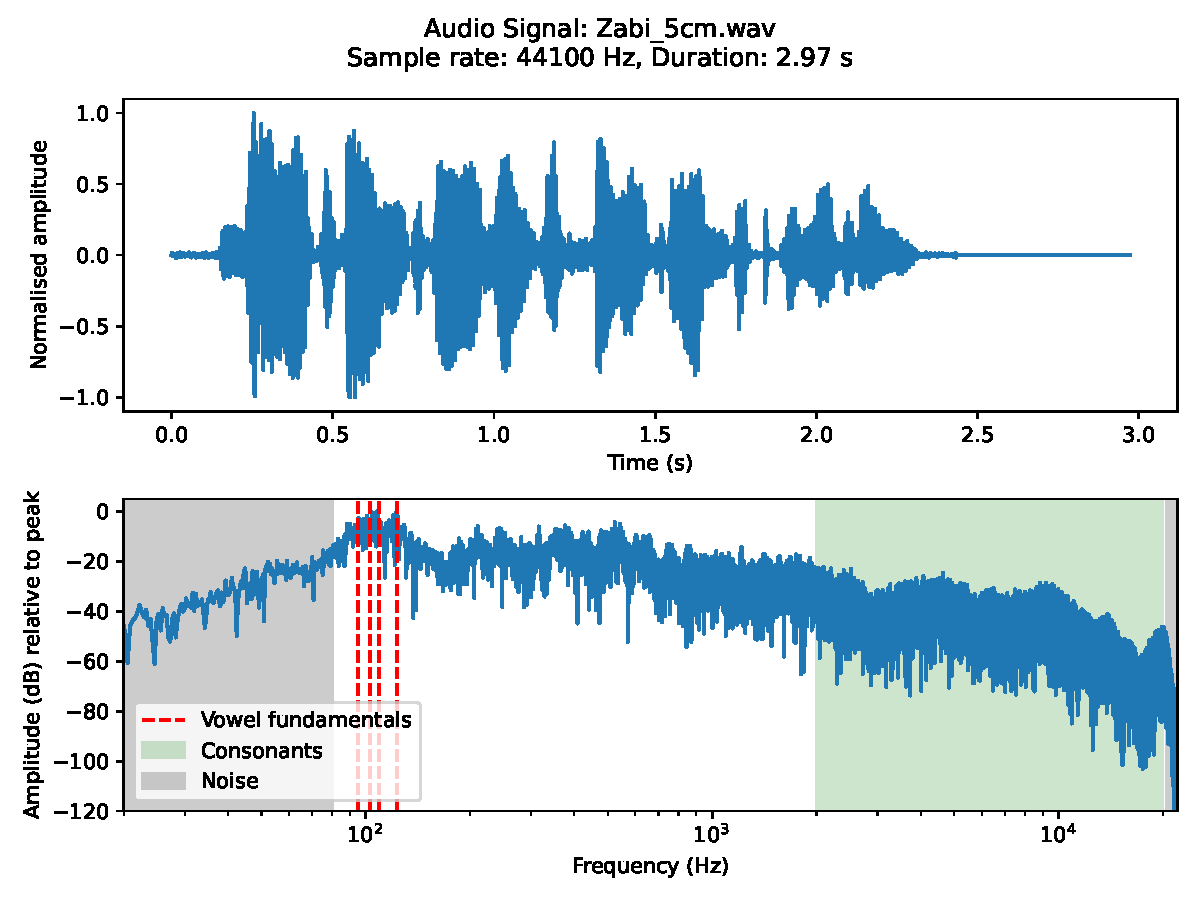
\includegraphics[width=0.88\linewidth]{Zabi_5cm.pdf}
  \caption{\SI{5}{\centi\metre} recording: normalised waveform (top) and
           spectrum (bottom) with vowel fundamentals (red), consonant range
           (green) and noise regions (grey) marked.}
  \label{fig:t1_5cm}
\end{figure}

\begin{figure}[htbp]
  \centering
  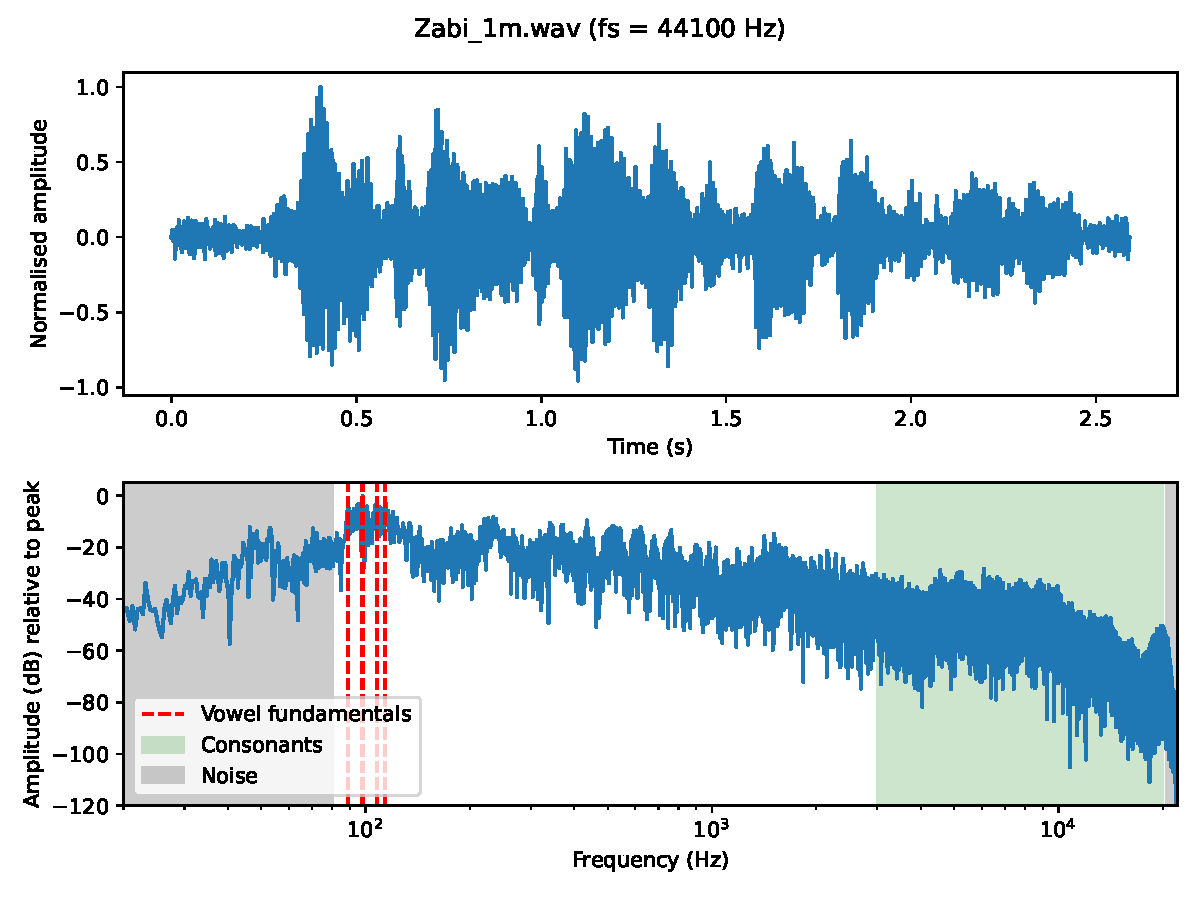
\includegraphics[width=0.88\linewidth]{Zabi_1m.pdf}
  \caption{\SI{1}{\metre} recording, marked in the same way as
           \cref{fig:t1_5cm}.}
  \label{fig:t1_1m}
\end{figure}

\paragraph{Time domain.}
The \SI{5}{\centi\metre} waveform (\cref{fig:t1_5cm}) has clearly separated
syllables with near-silent gaps between them. At \SI{1}{\metre}
(\cref{fig:t1_1m}) the gaps are filled in. The silent lead-in before the
speech sits at \SI{-41.6}{\decibel} relative to the peak at
\SI{5}{\centi\metre} but at \SI{-25.3}{\decibel} at \SI{1}{\metre}. Once both
files are normalised, the room noise is therefore about \SI{16}{\decibel}
louder relative to the voice at the larger distance.

\paragraph{Vowel fundamentals.}
Vowels are voiced, so each one produces a strong peak at the speaker's
fundamental, with its harmonics at integer multiples above it. Zabi has a male
speaking voice, so we looked for the first strong peaks above the noise region
in the region of \SIrange{85}{155}{\hertz}. At \SI{5}{\centi\metre} we marked
six peaks (\SIlist{88.7;95.3;100.6;104.7;108;122.5}{\hertz}). Each vowel is
spoken at a slightly different pitch, which is why they appear as separate
peaks rather than one. At \SI{1}{\metre} only four could be picked out
(\SIlist{89.2;98;107.7;114}{\hertz}). The two recordings are separate takes,
so the pitch of each vowel is slightly different, and at \SI{1}{\metre} the room
rumble in the same range fills the gaps between neighbouring peaks, so some of
them can no longer be told apart.

\paragraph{Consonants.}
Fricatives and plosives such as ``s'', ``f'' and ``t'' are bursts of turbulent
air with no fundamental, so their energy sits high in the spectrum where the
vowel harmonics have died away. Above about \SI{3}{\kilo\hertz} the spectrum
stops showing a regular harmonic comb and turns into a broad, noise-like
plateau, so we start the consonant range there. It extends up to
\SI{20}{\kilo\hertz}. The hump at \SIrange{17}{20}{\kilo\hertz} is still
\SIrange{16}{24}{\decibel} above the silent lead-in, so it is speech, and above
\SI{20}{\kilo\hertz} the spectrum falls off steeply. Both recordings use the
same range because it is the same speaker and sentence.

\paragraph{Noise.}
Two regions most likely contain only noise. Below \SI{80}{\hertz} is under
the lowest vowel fundamental, so it cannot be voice. It holds room rumble and,
in the \SI{5}{\centi\metre} recording, the low-frequency thumps of ``p'' and
``b'' pops. Above \SI{20.5}{\kilo\hertz} is beyond human hearing and inside the
recorder's anti-aliasing roll-off, so it carries no useful speech.

% =====================================================================
\section{Task 2: Spectral Enhancement}
\label{sec:task2}\label{sec:enhance}

Each recording is enhanced with a single gain curve $G$ built from
\cref{eq:ramp}:
\begin{equation}
  Y[k] = G[k]\,X[k],
  \qquad
  y[n] = \operatorname{Re}\!\left\{\mathrm{IFFT}\{Y[k]\}\right\},
  \label{eq:filter}
\end{equation}
\begin{equation}
  G =
  \underbrace{\ramp{60}{80}\,\bigl(1-\ramp{20000}{20500}\bigr)}_{\text{noise cuts}}
  \;\underbrace{\bigl(1 + 0.3\,\ramp{1500}{2000}\,(1-\ramp{5000}{6000})\bigr)}_{\text{presence, both files}}
  \;\underbrace{\bigl(1 + 0.4\,(1-\ramp{120}{150})\bigr)}_{\text{bass, \SI{1}{\metre} only}}
  \label{eq:gain}
\end{equation}
The output is renormalised to a peak of 1 and saved as a 32-bit float WAV.

\begin{table}[htbp]
  \centering
  \caption{Changes made to each recording in Task 2.}
  \label{tab:task2}
  \begin{tabular}{@{}llll@{}}
    \toprule
    Change & Band & Applied to & Reason \\
    \midrule
    Cut              & below \SI{80}{\hertz}          & both & rumble, and pops at \SI{5}{\centi\metre} \\
    Cut              & above \SI{20.5}{\kilo\hertz}   & both & noise region from Task 1 \\
    $\times1.3$ (\SI{+2.3}{\decibel}) & \SIrange{2}{5}{\kilo\hertz} & both & presence and intelligibility \\
    $\times1.4$ (\SI{+2.9}{\decibel}) & \SIrange{80}{120}{\hertz}   & \SI{1}{\metre} only & restore vowel fundamentals \\
    \bottomrule
  \end{tabular}
\end{table}

\paragraph{\SI{5}{\centi\metre}: pops.}
The risk at close range is plosive pops. The air blast from ``p'' and ``b''
hits the microphone and produces thumps below \SI{80}{\hertz}. The close
recording also already has a strong low end, so no bass is added. Cutting
below \SI{80}{\hertz} removes the pops without touching the voice, since the
lowest fundamental is \SI{88.7}{\hertz}. The ramp starts at \SI{60}{\hertz},
so the cut is fully in place before the voice begins.

\paragraph{\SI{1}{\metre}: room noise and lost bass.}
At \SI{1}{\metre} the voice is quieter relative to the room, and the direct
bass of the voice is weaker. However, the low end of the \SI{1}{\metre}
spectrum is not actually lower than at \SI{5}{\centi\metre}, because room noise
fills it in. \SI{81}{\percent} of the energy in the silent lead-in lies below
\SI{200}{\hertz}. That noise overlaps the vowel fundamentals, so only the part
below \SI{80}{\hertz} can be removed. Boosting the whole bass region would
mostly boost noise. The bass boost is therefore limited to the band below
\SI{120}{\hertz}, where the vowel fundamentals are strongest compared with the
noise, and it fades back to unity by \SI{150}{\hertz}. Our first version
boosted \SIrange{100}{300}{\hertz} by $\times2$, but it missed two of the four
fundamentals and made the silent parts noisier, so it was replaced.

\paragraph{Clarity.}
The \SIrange{2}{5}{\kilo\hertz} region holds the consonant detail that makes
speech intelligible and gives radio voices their ``presence''. It is lifted by
a modest \SI{2.3}{\decibel} in both recordings.
\Cref{fig:t2_5cm,fig:t2_1m} show the spectra before and after.

\begin{figure}[htbp]
  \centering
  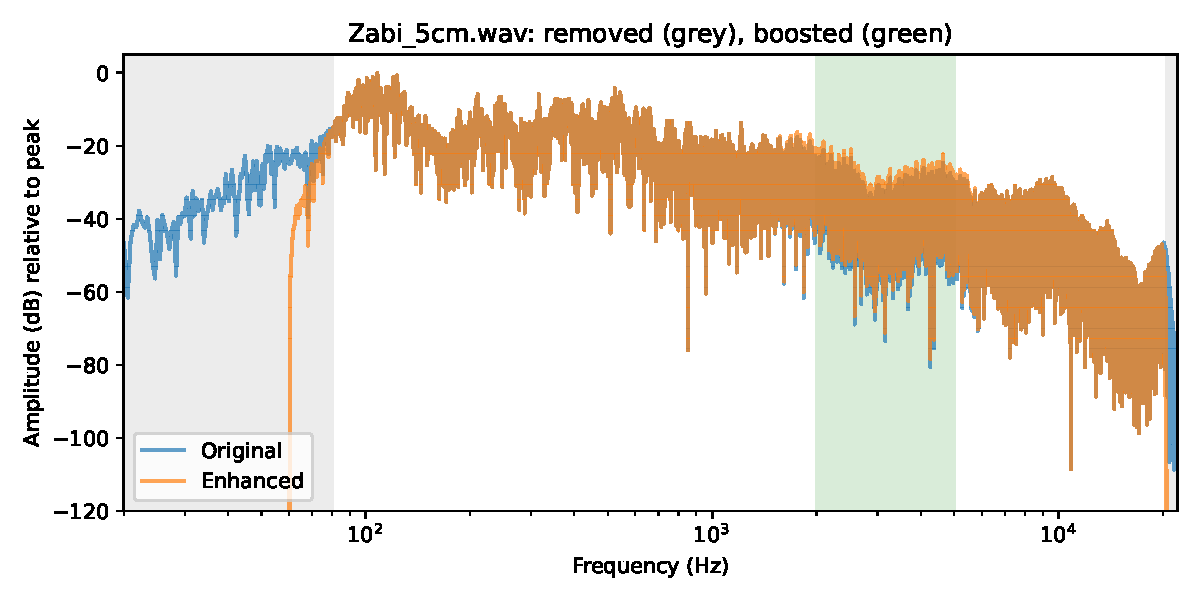
\includegraphics[width=0.85\linewidth]{Zabi_5cm_task2.pdf}
  \caption{\SI{5}{\centi\metre} recording before and after enhancement. Both
           curves use the original peak as \SI{0}{\decibel}.}
  \label{fig:t2_5cm}
\end{figure}

\begin{figure}[htbp]
  \centering
  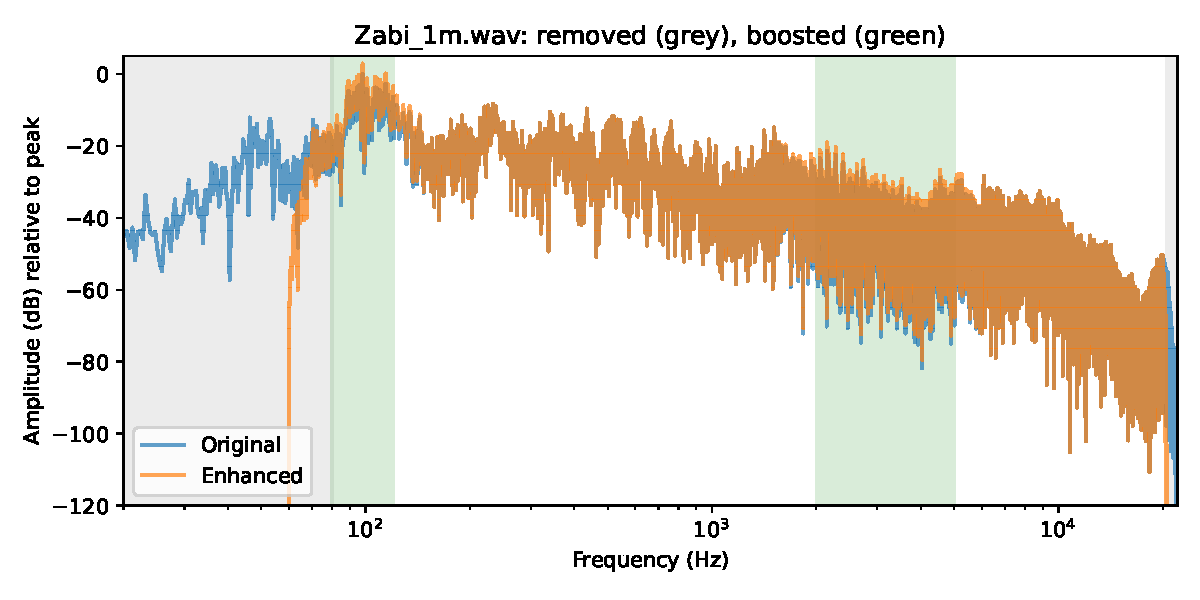
\includegraphics[width=0.85\linewidth]{Zabi_1m_task2.pdf}
  \caption{\SI{1}{\metre} recording before and after enhancement, with the
           extra \SIrange{80}{120}{\hertz} boost.}
  \label{fig:t2_1m}
\end{figure}

% =====================================================================
\section{Aural Exciter}
\label{sec:exciter}

We based our exciter on the Aphex block diagram from the brief and applied it
to the \SI{5}{\centi\metre} recording, after removing the pops and noise in
the same way as in \cref{sec:enhance}. Like the diagram, it has two
sidechains that are mixed back in with the original voice at the SUM block:
\begin{equation}
  y[n] = x[n] + \mathrm{mix}\cdot h[n] + \mathrm{bass\_mix}\cdot b[n],
  \label{eq:mix}
\end{equation}
where \texttt{mix} and \texttt{bass\_mix} are the two Mix controls in the
diagram and have the same names in our code.

In the Aural Exciter sidechain $h[n]$, the voice is high-passed and normalised
to a peak of 1 before going through a $\tanh$ nonlinearity, as suggested in
the brief:
\begin{equation}
  d[n] = \tanh\!\big( \mathrm{drive}\cdot x_{\mathrm{hp}}[n] \big),
  \label{eq:nonlin}
\end{equation}
which creates harmonics of the voice. Because speech contains lots of
frequencies at once, the $\tanh$ also creates sum and difference frequencies
between them that can land anywhere in the spectrum, so we band-pass $d[n]$
again to keep only the harmonics we want, as the brief describes. The Big
Bottom sidechain $b[n]$ works in a similar way on the low end, where the
voice below \SI{190}{\hertz} is put through $\tanh(3x)$. This squashes loud
bass more than quiet bass, so it acts like the dynamics processor in the
diagram. All of the filters are done by multiplying the FFT and taking the
IFFT, with sloped edges instead of hard cuts to avoid ringing.

\begin{table}[htbp]
  \centering
  \caption{Exciter settings and how much each version changed the voice.}
  \label{tab:exciter}
  \begin{tabular}{@{}lcc@{}}
    \toprule
    & v1 (first try) & v2 (final) \\
    \midrule
    High-pass into $\tanh$ & \SI{800}{\hertz} & \SI{3}{\kilo\hertz} \\
    Harmonics kept & all & \SIrange{4}{12}{\kilo\hertz} \\
    \texttt{drive} & 5 & 5 \\
    \texttt{mix} & 0.3 & 0.15 \\
    \texttt{bass\_mix} & 0 & 0.1 \\
    \midrule
    Change at \SIrange{80}{190}{\hertz} & \SI{0}{\decibel} & \SI{+2.2}{\decibel} \\
    Change at \SIrange{4}{10}{\kilo\hertz} & \SI{+6.7}{\decibel} & \SI{+2.8}{\decibel} \\
    Change at \SIrange{12}{20}{\kilo\hertz} & \SI{+7.5}{\decibel} & \SI{0}{\decibel} \\
    \bottomrule
  \end{tabular}
\end{table}

Our first version (v1) boosted everything above \SI{800}{\hertz} by
\SIrange{6}{9}{\decibel} (\cref{fig:exciter_change}), which made the voice
sound harsh. Because we didn't filter after the $\tanh$, it also put energy
back below \SI{80}{\hertz}, where we had just removed the pops. For v2, we
moved the high-pass up to \SI{3}{\kilo\hertz} and only kept harmonics between
\SI{4}{\kilo\hertz} and \SI{12}{\kilo\hertz}. This band is centred around
\SI{6}{\kilo\hertz}, where the brief says the ear is most sensitive. We also
halved \texttt{mix} and added a small amount of Big Bottom bass.
\Cref{fig:exciter_v2} shows that v2 only adds content in those two bands.
When listening back, v1 sounds much sharper than v2. This is most likely
because v1 raises the \SIrange{12}{20}{\kilo\hertz} range by
\SI{7.5}{\decibel}, which is where the hissy ``s'' and ``t'' sounds sit, and
keeps every harmonic the $\tanh$ creates at twice the mix level. v2 leaves
that range untouched, so its added brightness stays in the region the ear is
most sensitive to without making those sounds piercing.

One thing we noticed is that with \texttt{drive} at 5, the $\tanh$ barely
bends the signal, since only about \SI{1}{\percent} of samples are affected.
This means most of v2's boost is really the existing
\SIrange{4}{12}{\kilo\hertz} content turned up, with only some new harmonics
on top. We tried a version with a drive of 20, which produced almost pure
harmonics, but it sounded squawky, so we kept v2.

\begin{figure}[htbp]
  \centering
  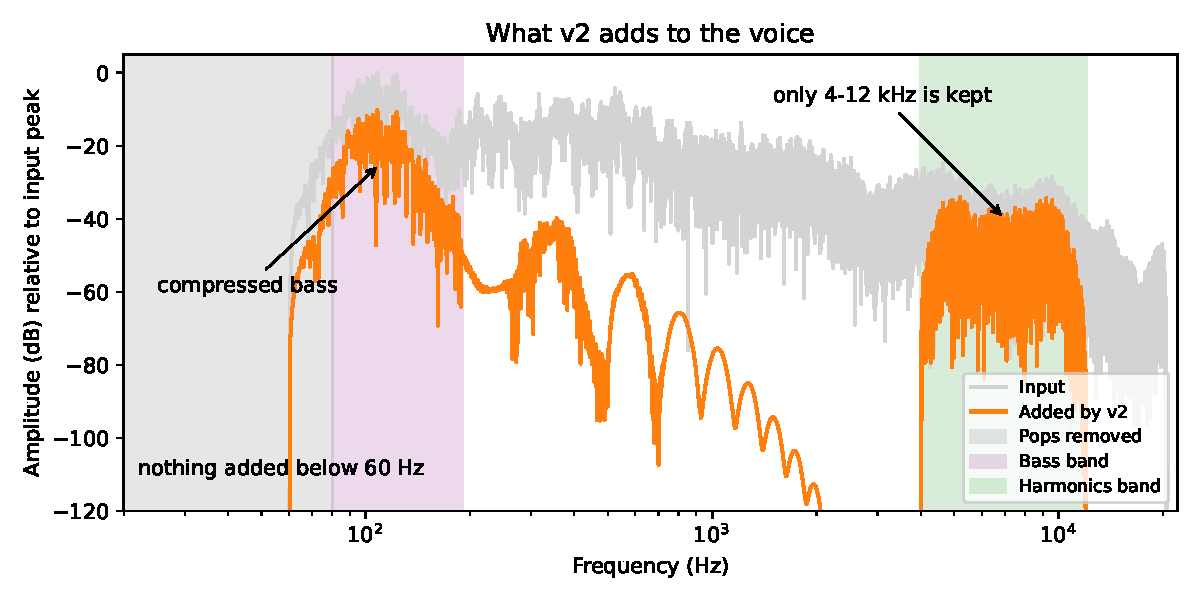
\includegraphics[width=\linewidth]{task3_v2.pdf}
  \caption{What exciter v2 adds to the voice, drawn over the input spectrum.}
  \label{fig:exciter_v2}
\end{figure}

\begin{figure}[htbp]
  \centering
  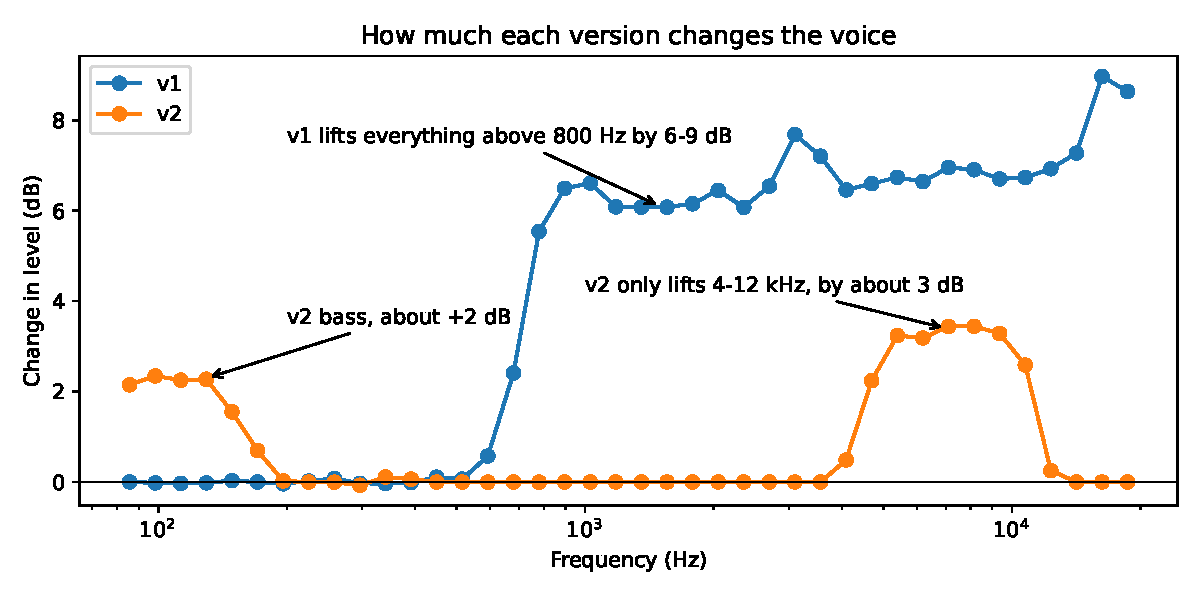
\includegraphics[width=\linewidth]{task3_change.pdf}
  \caption{How much each version changes the voice level, averaged over 40
           log-spaced bands.}
  \label{fig:exciter_change}
\end{figure}

% =====================================================================
\section{Conclusion}
\label{sec:conclusion}

Moving from \SI{5}{\centi\metre} to \SI{1}{\metre} raised the room-noise floor
by about \SI{16}{\decibel} relative to the voice. Most of that noise is
below \SI{200}{\hertz}, so it overlaps the vowel fundamentals and can only be
partly removed with FFT gains. At close range the main problem was pops below
\SI{80}{\hertz}, which could be removed cleanly. Ramped gain edges were
essential, because hard edges made the enhanced voice ring. For the exciter,
limiting both the input to the nonlinearity and the harmonics kept from it was
what turned a harsh first attempt into a usable design. The final exciter lifts
\SIrange{4}{12}{\kilo\hertz} by about \SI{3}{\decibel} while changing the
overall level by under \SI{1}{\decibel}.

% =====================================================================
\section*{Acknowledgement of GenAI Use}
We used Claude (Claude Opus 5.5, Anthropic) to review our code against the
brief, check the measurements quoted in this report, and help structure and
word the report text. We made the recordings, wrote the initial code, chose
the filter bands and exciter settings, and made all listening judgements
ourselves. Any code suggestions were checked and simplified by us, and we can
both explain every line of the submitted code.

% =====================================================================
\appendix
\section{Python Code}
\label{app:code}

\subsection*{\texttt{task1.py}}
\begin{lstlisting}
import os
import numpy as np
import matplotlib.pyplot as plt
from scipy.io import wavfile

os.chdir(os.path.dirname(os.path.abspath(__file__)))  # find the wav files wherever the script is run from

# Regions chosen by eye
# same speaker and sentence, so the consonants sit in the same range at both distances
marks = {
    "Zabi_5cm.wav": {"vowels": [88.7, 95.3, 100.6, 104.7, 108, 122.5], "consonants": (3000, 20000), "noise": [(20, 80), (20500, 22050)]},
    "Zabi_1m.wav":  {"vowels": [89.2, 98, 107.7, 114],  "consonants": (3000, 20000), "noise": [(20, 80), (20500, 22050)]},
}

# Main Loop
for filename, m in marks.items():
    fs, x = wavfile.read(filename)
    x = x[:, 0]  # stereo file, both channels are the same
    x = x / np.max(np.abs(x))  # normalise to +-1
    x = np.trim_zeros(x, "b")  # trim trailing zeros added by garageband  ## "b" given in numpy doc just to cut trailing

    N = len(x)
    t = np.arange(N) / fs #for time axis

    # spectrum up to Nyquist, skipping the DC bin so the log axis works
    X = np.abs(np.fft.fft(x)[1:N // 2])
    f = np.arange(1, N // 2) * fs / N
    XdB = 20 * np.log10(X / np.max(X)) #dB relative to peak

    # plotting
    fig, (ax1, ax2) = plt.subplots(2, 1, figsize=(8, 6))
    fig.suptitle(f"{filename} (fs = {fs} Hz)")
    ax1.plot(t, x)
    ax1.set_xlabel("Time (s)")
    ax1.set_ylabel("Normalised amplitude")

    ax2.plot(f, XdB)
    ax2.set_xscale("log")
    ax2.set_xlim(20, fs / 2)  # audible range up to Nyquist
    ax2.set_ylim(-120, 5)
    ax2.set_xlabel("Frequency (Hz)")
    ax2.set_ylabel("Amplitude (dB) relative to peak")
    ax2.vlines(m["vowels"], -120, 5, colors="r", linestyles="--", label="Vowel fundamentals")
    ax2.axvspan(*m["consonants"], color="g", alpha=0.2, label="Consonants")
    low, high = m["noise"]
    ax2.axvspan(*low, color="grey", alpha=0.4, label="Noise")
    ax2.axvspan(*high, color="grey", alpha=0.4)
    ax2.legend(loc="lower left")
    fig.tight_layout()
    fig.savefig(filename.replace(".wav", ".pdf"))  

plt.show()
\end{lstlisting}

\subsection*{\texttt{task2.py}}
\begin{lstlisting}
import os
import numpy as np
import matplotlib.pyplot as plt
from scipy.io import wavfile

os.chdir(os.path.dirname(os.path.abspath(__file__)))  # find the wav files wherever the script is run from

filenames = ["Zabi_5cm.wav", "Zabi_1m.wav"]


# gain that goes from 0 at f0 up to 1 at f1, so 1 - ramp is a lowpass (same as task 3)
# slopes instead of hard steps because hard steps in the gain made the voice ring
# f is the frequency axis of the file being processed, set in the loop below
def ramp(f0, f1):
    return np.clip((f - f0) / (f1 - f0), 0, 1)


for filename in filenames:
    fs, x = wavfile.read(filename)
    x = x[:, 0]  # stereo file, both channels are the same
    x = x / np.max(np.abs(x))  # normalise to +-1
    x = np.trim_zeros(x, "b")  # trim trailing zeros added by garageband  ## "b" given in numpy doc just to cut trailing
    N = len(x)

    #fft
    X = np.fft.fft(x)

    # frequency of each bin, the second half is a mirror of the first half
    # so fold it back so both halves get changed the same
    f = np.arange(N) * fs / N
    f = np.minimum(f, fs - f)

    # remove everything below 80 Hz (rumble, and pops for the 5cm one)
    # and the upper noise margin identified in task 1, above 20.5 kHz
    G = ramp(60, 80) * (1 - ramp(20000, 20500))

    # boost 2-5 kHz to make the voice clearer
    G *= 1 + 0.3 * ramp(1500, 2000) * (1 - ramp(5000, 6000))  # x1.3 is about +2.3 dB

    # boost bass for 1m only because bass is lost with distance
    # 5cm already has loads of bass (proximity effect)
    # only below 120 Hz where the vowel fundamentals are (89-114 Hz in task 1),
    # the room noise is worst compared to the voice at 120-200 Hz so that is left alone
    if filename == "Zabi_1m.wav":
        G *= 1 + 0.4 * (1 - ramp(120, 150))  # x1.4 is about +3 dB

    Y = X * G

    #ifft back to time domain
    y = np.real(np.fft.ifft(Y))  # imaginary part is basically 0
    y = y / np.max(np.abs(y))  # normalise again so it doesnt clip

    wavfile.write(filename.replace(".wav", "_enhanced.wav"), fs, y.astype(np.float32))

    #plot before and after
    half = N // 2
    mag_before = np.abs(X[1:half])
    mag_after = np.abs(Y[1:half])
    ref = np.max(mag_before)  # same reference for both so the plot shows the real change
    dB_before = 20 * np.log10(mag_before / ref + 1e-12)
    dB_after = 20 * np.log10(mag_after / ref + 1e-12)

    fig, ax = plt.subplots(figsize=(8, 4))
    ax.plot(f[1:half], dB_before, label="Original", alpha=0.7)
    ax.plot(f[1:half], dB_after, label="Enhanced", alpha=0.7)

    # shade the bands that were changed, grey = removed, green = boosted
    ax.axvspan(20, 80, color="grey", alpha=0.15)
    ax.axvspan(20500, fs / 2, color="grey", alpha=0.15)
    if filename == "Zabi_1m.wav":
        ax.axvspan(80, 120, color="green", alpha=0.15)
    ax.axvspan(2000, 5000, color="green", alpha=0.15)

    ax.set_xscale("log")
    ax.set_xlim(20, fs / 2)
    ax.set_ylim(-120, 5)
    ax.set_xlabel("Frequency (Hz)")
    ax.set_ylabel("Amplitude (dB) relative to peak")
    ax.set_title(filename + ": removed (grey), boosted (green)")
    ax.legend(loc="lower left")
    fig.tight_layout()
    fig.savefig(filename.replace(".wav", "_task2.pdf"))

plt.show()
\end{lstlisting}

\subsection*{\texttt{task3.py}}
\begin{lstlisting}
import os
import numpy as np
import matplotlib.pyplot as plt
from scipy.io import wavfile

# aural exciter based on the aphex block diagram in the brief
# exciter part: highpass -> tanh makes harmonics -> only keep some of them -> mix back in
# big bottom part: lowpass -> tanh squashes it like a compressor -> mix back in
# all the filtering is done by multiplying the fft and then doing the ifft (like task 2)

os.chdir(os.path.dirname(os.path.abspath(__file__)))  # find the wav files wherever the script is run from

fs, x = wavfile.read("Zabi_5cm.wav")
x = x[:, 0]  # stereo file, both channels are the same
x = x / np.max(np.abs(x))  # normalise to +-1
x = np.trim_zeros(x, "b")  # trim trailing zeros added by garageband
N = len(x)

# frequency of each bin, folded like in task 2 so both halves get changed the same
f = np.arange(N) * fs / N
f = np.minimum(f, fs - f)


# gain that goes from 0 at f0 up to 1 at f1, so 1 - ramp is a lowpass
# used a slope instead of a hard cut because hard cuts can cause ringing
def ramp(f0, f1):
    return np.clip((f - f0) / (f1 - f0), 0, 1)


#fft
X = np.fft.fft(x)

# remove pops below 80 Hz and noise above 20.5 kHz first, same cuts as task 2
# task 2's 2-5 kHz boost is left out, making the voice clearer is the exciter's job here
X = X * ramp(60, 80) * (1 - ramp(20000, 20500))
x = np.real(np.fft.ifft(X))

# big bottom, lowpass then tanh squashes the loud bits like a compressor
# tanh puts a bit back below 80 Hz, so the pop cut is done again afterwards
# it's the same for every version so it only gets worked out once
low = np.real(np.fft.ifft(X * (1 - ramp(150, 190))))
low = low / np.max(np.abs(low))
bass = np.real(np.fft.ifft(np.fft.fft(np.tanh(3 * low)) * ramp(60, 80)))


# hp = highpass gain, band = which harmonics to keep, drive = how hard tanh gets pushed,
# mix and bass_mix = how much of each part gets added back
# returns only the part that gets added to the voice
def exciter(hp, band, drive, mix, bass_mix):
    # highpass, then normalise so drive does the same thing every time
    side = np.real(np.fft.ifft(X * hp))
    side = side / np.max(np.abs(side))

    # tanh makes the harmonics, its symmetric so only odd ones (3rd, 5th...)
    harm = np.tanh(drive * side)

    # only keep the harmonics inside the band
    harm = np.real(np.fft.ifft(np.fft.fft(harm) * band))
    harm = harm / np.max(np.abs(harm))

    return mix * harm + bass_mix * bass


# v1 first try: highpass at 800 Hz and keep all the harmonics (band = 1)
added1 = exciter(ramp(600, 800), 1, 5, 0.3, 0)

# v2: v1 boosts everything above 800 Hz (12-20 kHz goes up about 7 dB) and puts stuff back
# below 80 Hz where i'd removed the pops (see figure 1)
# so the highpass is moved up to 3 kHz, only harmonics from 4-12 kHz are kept,
# plus a bit of bass to try the big bottom side of the aphex diagram
hp2 = ramp(2000, 3000)
band2 = ramp(4000, 5000) * (1 - ramp(10000, 12000))  # highpass * lowpass = bandpass
added2 = exciter(hp2, band2, 5, 0.15, 0.1)

y1 = x + added1
y2 = x + added2

# save them so i can listen, normalised so they dont clip
out1 = y1 / np.max(np.abs(y1))
out2 = y2 / np.max(np.abs(y2))
wavfile.write("Zabi_5cm_exciter_v1_initial.wav", fs, out1.astype(np.float32))
wavfile.write("Zabi_5cm_exciter_v2_final.wav", fs, out2.astype(np.float32))

#plotting
half = N // 2
fp = f[1:half]  # skip DC for the log axis
ref = np.max(np.abs(X[1:half]))  # 0 dB = input peak so all the curves can be compared


def dB(s):
    mag = np.abs(np.fft.fft(s)[1:half])
    return 20 * np.log10(mag / ref + 1e-12)


x_dB = dB(x)

# figures 1 and 2: what each version adds, drawn over the input so you can see how loud it is
def plot_added(added, version, colour):
    fig, ax = plt.subplots(figsize=(8, 4))
    ax.plot(fp, x_dB, label="Input", color="lightgrey")
    ax.plot(fp, dB(added), label=f"Added by {version}", color=colour)
    ax.axvspan(20, 80, color="grey", alpha=0.2, label="Pops removed")
    ax.set_xscale("log")
    ax.set_xlim(20, fs / 2)
    ax.set_ylim(-120, 5)
    ax.set_xlabel("Frequency (Hz)")
    ax.set_ylabel("Amplitude (dB) relative to input peak")
    ax.set_title(f"What {version} adds to the voice")
    return fig, ax


arrow = dict(arrowstyle="->")

fig1, ax1 = plot_added(added1, "v1", "C0")
ax1.annotate("almost as loud as the voice\nabove 800 Hz, sounds harsh", xy=(8000, -30), xytext=(1000, -95), arrowprops=arrow)
ax1.annotate("energy put back\nwhere the pops were", xy=(45, -50), xytext=(22, -100), arrowprops=arrow)
ax1.legend(loc="upper right", fontsize="small")

fig2, ax2 = plot_added(added2, "v2", "C1")
ax2.axvspan(80, 190, color="purple", alpha=0.15, label="Bass band")
ax2.axvspan(4000, 12000, color="green", alpha=0.15, label="Harmonics band")
ax2.annotate("only 4-12 kHz is kept", xy=(7000, -40), xytext=(1500, -8), arrowprops=arrow)
ax2.annotate("compressed bass", xy=(110, -25), xytext=(25, -60), arrowprops=arrow)
ax2.text(22, -110, "nothing added below 60 Hz")
ax2.legend(loc="lower right", fontsize="small")

# figure 3: how much each version changes the level of the voice, averaged over 40 bands
# so the curves are smooth enough to compare (starts at 80 Hz, below that the input is cut)
edges = np.geomspace(80, 20000, 41)
centres = np.sqrt(edges[:-1] * edges[1:])  # middle of each band on a log axis


def band_power(s):
    P = np.abs(np.fft.fft(s)[1:half]) ** 2
    return np.array([P[(fp >= lo) & (fp < hi)].mean() for lo, hi in zip(edges[:-1], edges[1:])])


Px = band_power(x)
fig3, ax3 = plt.subplots(figsize=(8, 4))
ax3.plot(centres, 10 * np.log10(band_power(y1) / Px), "o-", label="v1")
ax3.plot(centres, 10 * np.log10(band_power(y2) / Px), "o-", label="v2")
ax3.axhline(0, color="k", linewidth=0.5)
ax3.annotate("v1 lifts everything above 800 Hz by 6-9 dB", xy=(1500, 6.1), xytext=(200, 7.5), arrowprops=arrow)
ax3.annotate("v2 only lifts 4-12 kHz, by about 3 dB", xy=(7000, 3.4), xytext=(1000, 4.2), arrowprops=arrow)
ax3.annotate("v2 bass, about +2 dB", xy=(130, 2.3), xytext=(200, 3.5), arrowprops=arrow)
ax3.set_xscale("log")
ax3.set_xlabel("Frequency (Hz)")
ax3.set_ylabel("Change in level (dB)")
ax3.set_title("How much each version changes the voice")
ax3.legend(loc="upper left")

for fig in [fig1, fig2, fig3]:
    fig.tight_layout()
fig1.savefig("task3_v1.pdf")
fig2.savefig("task3_v2.pdf")
fig3.savefig("task3_change.pdf")
plt.show()
\end{lstlisting}

\end{document}
